\documentclass[11pt]{article}

\usepackage[a4paper,margin=1in]{geometry}
\usepackage{microtype}
\usepackage{amsmath,amssymb,amsfonts}
\usepackage{hyperref}
\usepackage{float}
\usepackage{placeins}
\usepackage{amsmath}
\usepackage{booktabs} 
\usepackage{array,booktabs,tabularx}
\usepackage{tikz}
\usepackage{indentfirst}
\usetikzlibrary{arrows.meta,calc,angles,quotes}

\newcolumntype{L}{>{\raggedright\arraybackslash}X}
\newcommand{\sech}{\operatorname{sech}}


\numberwithin{equation}{section}

\title{Unimetry: A Phase-Space Reformulation of Special Relativity}
\author{Timur Abizgeldin\\ \small Independent researcher, Austria\\ \small \texttt{timurabizgeldin@gmail.com}}
\date{\today}


% --- Unimetry macros ---
\usepackage{tikz}
\usetikzlibrary{arrows.meta,positioning,calc}
\providecommand{\bi}{\mathbf{i}}
\providecommand{\bj}{\mathbf{j}}
\providecommand{\bk}{\mathbf{k}}
\providecommand{\uhat}{\hat{\mathbf u}}
\providecommand{\rotor}[2]{\cos\frac{#2}{2} + #1\,\sin\frac{#2}{2}}

\begin{document}
\maketitle
\begin{abstract}
We propose a compact reformulation of special relativity in which spacetime measures (time and length) are treated as phase velocities, defined as directional derivatives of a single underlying parameter, the flow $\boldsymbol{\chi}\in\mathbb{H}$. In this framework, the observable Minkowski interval emerges as a conserved quantity under a change of parameter from the phase coordinate $\chi$ to the observer’s proper time $\tau$. Familiar relativistic effects, such as time dilation, the Lorentz factor, the Doppler shift, and relativistic velocity composition, arise as elementary projections and rotations within a Euclidean phase plane. Hyperbolic features of Lorentz kinematics reappear after a reparametrization of time, yielding the classical relations without altering empirical content. We provide closed-form derivations for the longitudinal and transverse Doppler effects, prove a lemma equating the total flow speed to the conserved Minkowski norm, and outline connections to gauge phases, rapidity, and a cosmological time gauge. Composition of non-collinear boosts (quaternionic $d$-rotations in $\mathbb{H}$) yields a Wigner rotation; in the continuous limit, this gives Thomas precession. Both effects emerge as purely kinematical consequences of the quaternionic phase formalism. The approach is advantageous for applications – especially in modeling non-collinear acceleration of particle beams – where it replaces matrix diagonalizations with algebraic rotor compositions and improves numerical stability.
\end{abstract}

\paragraph{Keywords:} special relativity; phase; rapidity; Doppler shift; Lorentz factor; Wigner rotation; Thomas precession; phase parametrization.

\paragraph{MSC (2020):} 83A05; 70A05. % (Consider also PACS: 03.30.+p; 04.20.Cv.)

%1 ====================================================================

\section{Introduction}
In classical physics, space and time are taken as absolute and independent entities – a view deeply rooted in Newtonian tradition and characterizing most formulations prior to the early twentieth century. Special relativity revolutionized this perspective by demonstrating that both are intertwined and relative, depending on the observer’s state of motion. Yet most conventional treatments still regard spacetime coordinates as fundamental ingredients, with subsequent physical phenomena described in their terms.

This work adopts an alternative viewpoint: instead of starting from space and time as primitives, we treat observed spacetime quantities as derived projections of an underlying phenomenon – a continuous “flow” parameter $\boldsymbol{\chi}$ in quaternionic space $\mathbb{H}$. In this approach, the flow constitutes the primary structure, carrying both local geometric and dynamical information; observable temporal and spatial measures emerge from its decomposition relative to an observer’s frame.

This reformulation allows us to re-express relativistic effects – such as time dilation, Lorentz contraction, and the Doppler shift – as geometric consequences of rotations and projections in phase space, with quaternion algebra naturally unifying spatial rotations and boosts. The speed of light, in this setting, arises as the constant magnitude of the flow measured locally.

The proposal reorganizes familiar relations in a language aligned with quantum-rotor kinematics, demonstrating the physical equivalence between Lorentz transformations and Euclidean rotations under proper-time parametrization. We realize the phase kinematics with quaternionic rotors
\[
d=\cos\frac{\psi}{2}+\hat{\mathbf u}\,\sin\frac{\psi}{2}.
\]
Throughout, we use three angles – intrinsic ($\zeta$), gravitational ($\phi$), and kinematic ($\vartheta$) – and, when focusing on special relativity (SR), we state the corresponding simplification explicitly. We emphasize that no modification of Einstein’s dynamics is proposed; all results are kinematical identities obtained by a change of parameter.

\paragraph{Notation.} Tildes, dots, and primes denote derivatives with respect to the phase parameter, proper time, and spatial arclength:
\[
\tilde{X}:=\frac{dX}{d\chi},\qquad \dot{X}:=\frac{dX}{d\tau},\qquad X':=\frac{dX}{dl}.
\]

\begin{table}[t]
\centering
\caption{Derivatives notation used in the paper.}
\label{tab:notation-phase}
\setlength{\tabcolsep}{6pt}\renewcommand{\arraystretch}{1.1}
\begin{tabularx}{\linewidth}{@{} l L @{}}
\toprule
\textbf{Symbol} & \textbf{Meaning} \\
\midrule
$\tilde{X}$ & Phase-parameter derivative or phase-normalized quantity; precise meaning is given at first occurrence. \\
$\dot{X}$ & Proper-time derivative $dX/d\tau$ (lab-time derivatives are written $dX/dt$ explicitly). \\
$X'$ & Derivative with respect to spatial arclength $l$ or value in a primed inertial frame (as stated locally). \\
\bottomrule
\end{tabularx}
\end{table}

We use $\mathtt{c}$ for the speed of light; $\beta:=v/\mathtt{c}$, $\gamma:=1/\sqrt{1-\beta^2}$, and rapidity defined by $\tanh\eta=\beta$. The subscript $l$ in $dx_l$ denotes spatial components, with $l=1,2,3$ a Cartesian index.

%1.1 ====================================================================
\subsection[Flow and phase 1-form]{Flow and phase 1-form}
Let $\Phi:\mathcal E\to\mathbb R$ be a scalar \emph{phase potential} on a (possibly infinite-dimensional) Euclidean/Hilbert proto-space $(\mathcal E,\langle\cdot,\cdot\rangle)$. 
Define the phase 1-form $\alpha:=d\Phi$ and the associated \emph{flow vector} $\boldsymbol\chi:=\nabla\Phi$, where the gradient is taken with respect to $\langle\cdot,\cdot\rangle$.

Fix an observer’s orthonormal spatial triad $\{\mathbf e_1,\mathbf e_2,\mathbf e_3\}\subset\mathcal E$ and let $S=\mathrm{span}\{\mathbf e_1,\mathbf e_2,\mathbf e_3\}$ with orthogonal projectors $P_S$ and $P_{S^\perp}$. Decompose
\[
\boldsymbol\chi=\boldsymbol\chi_S+\boldsymbol\chi_\perp,\qquad
\boldsymbol\chi_S:=P_S\boldsymbol\chi,\quad 
\boldsymbol\chi_\perp:=P_{S^\perp}\boldsymbol\chi.
\]
Define observable spatial components and the orthogonal magnitude
\[
\ell_i:=\langle\boldsymbol\chi,\mathbf e_i\rangle,\qquad 
\mathbf l:=\sum_{i=1}^3 \ell_i\,\mathbf e_i,\qquad 
t:=\|\boldsymbol\chi_\perp\|=\sqrt{\|\boldsymbol\chi\|^2-\|\boldsymbol\chi_S\|^2},
\]
and, when $t>0$, the unit direction $\mathbf e_t:=\boldsymbol\chi_\perp/\|\boldsymbol\chi_\perp\|$.
Then the full phase angle $\Theta$ and the spatial direction $\mathbf u$ used throughout are
\[
\cos\Theta=\frac{t}{\|\boldsymbol\chi\|},\qquad 
\sin\Theta=\frac{\|\mathbf l\|}{\|\boldsymbol\chi\|},\qquad 
\mathbf u=\frac{\mathbf l}{\|\mathbf l\|}\quad(\|\mathbf l\|>0).
\]
Thus the observable space is a 3-manifold embedded in a (minimum) 4-dimensional flow manifold; the quaternion algebra then simplifies operations on flows relative to the lab triad.

% ============================Minkowski metric derivation========================================

\subsection[Minkowski metric derivation]{Minkowski metric derivation}

Let $A$ be an observer with orthonormal spatial triad $\{\mathbf e_1^A,\mathbf e_2^A,\mathbf e_3^A\}$,
spatial subspace $S^A=\mathrm{span}\{\mathbf e_i^A\}$, and orthogonal projectors
$P_{S^A},P_{(S^A)^\perp}$.
Define the observer’s time direction $\mathbf e_t^A$ as the unit vector along $(S^A)^\perp$.
For any object with flow $\boldsymbol\chi$ set $\widehat{\mathbf F}:=\boldsymbol\chi/\|\boldsymbol\chi\|$.

\paragraph{Observer--object (relative) angle.}
Project $\widehat{\mathbf F}$ onto $A$’s split:
\[
\widehat{\mathbf F}
= (\widehat{\mathbf F}\!\cdot\!\mathbf e_t^A)\,\mathbf e_t^A
+ P_{S^A}\widehat{\mathbf F}
= \cos\vartheta_{\,\!|\!A}\,\mathbf e_t^A
+ \sin\vartheta_{\,\!|\!A}\,\mathbf u_{\,\!|\!A},
\]
where
\[
\cos\vartheta_{\,\!|\!A} \;:=\; \widehat{\mathbf F}\!\cdot\!\mathbf e_t^A,\qquad
\sin\vartheta_{\,\!|\!A} \;:=\; \big\|P_{S^A}\widehat{\mathbf F}\big\|,\qquad
\mathbf u_{\,\!|\!A} \;:=\; \frac{P_{S^A}\widehat{\mathbf F}}{\|P_{S^A}\widehat{\mathbf F}\|} \in S^A.
\]
\emph{Important:} this $\vartheta_{\,\!|\!A}$ is the \textbf{observer–object angle}. In general it is not the same as the “full phase angle” $\Theta$ we defined before, because
$\Theta$ is built from the object’s own split (its “self time” direction), whereas $\vartheta_{\,\!|\!A}$ is built from the \emph{observer’s} split. They coincide only in the co–moving case when the time directions agree.

\paragraph{Operational kinematics in $A$’s frame.}
Let $dt_A$ be $A$’s lab time, $d\mathbf x_{|\!A}\in S^A$ the object’s spatial shift measured by $A$, and $d\tau$ the object’s proper time. Then, exactly as in the single–frame picture,
\[
\frac{d\tau}{dt_A} \;=\; \cos\vartheta_{\,\!|\!A},\qquad
\frac{\|d\mathbf x_{|\!A}\|}{c\,dt_A} \;=\; \sin\vartheta_{\,\!|\!A}.
\]
By the elementary identity $\cos^2\!+\sin^2\!=1$,
\[
\boxed{\; c^2\,d\tau^2 \;=\; c^2\,dt_A^2 \;-\; \|d\mathbf x_{|\!A}\|^2 \;}
\]
which is precisely the Minkowski interval, now expressed using the \emph{observer–object} angle.

% ============================Symmetry========================================

\subsection[Symmetry]{Symmetry}

\paragraph{Two objects $A$ and $B$ (symmetry).}
Repeat the same construction in $B$’s frame to get
\[
\frac{d\tau_A}{dt_B}=\cos\vartheta_{A\,|\!B},\qquad
\frac{\|d\mathbf x_{A\,|\!B}\|}{c\,dt_B}=\sin\vartheta_{A\,|\!B},\qquad
c^2 d\tau_A^2=c^2 dt_B^2-\|d\mathbf x_{A\,|\!B}\|^2.
\]
Thus the mechanism is isotropic and frame–symmetric: swapping “who projects whom”
just swaps $(\mathbf e_t,S)$, while the Minkowski form is unchanged.

\paragraph{When do $\vartheta_{\,\!|\!A}$ and $\Theta$ match?}
Let $\Theta$ be the angle built from the object’s own split (its self time direction $\mathbf e_t^{\rm self}$). Then $\vartheta_{\,\!|\!A}=\Theta$ iff $\mathbf e_t^A=\mathbf e_t^{\rm self}$, i.e. in the co–moving case. In all other cases the two angles differ: one is an \emph{observer–relative} tilt, the other is a \emph{self–relative} tilt.

\paragraph{Velocity dictionary (in $A$’s frame).}
\[
\beta_{\,\!|\!A}:=\frac{\|d\mathbf x_{|\!A}\|}{c\,dt_A}=\sin\vartheta_{\,\!|\!A},\qquad
\gamma_{\,\!|\!A}:=\frac{dt_A}{d\tau}=\sec\vartheta_{\,\!|\!A}.
\]
All familiar SR relations are recovered by replacing the absolute angle with the
observer–object angle $\vartheta_{\,\!|\!A}$.

\subsection{Intrinsic metric of the object}\label{sec:intrinsic-metric}

In the flow-based description an object is a collection of elementary ``streamlets'' (fragments of phase flow). Each streamlet carries
(i) a budget angle $\Theta_a\in[0,\tfrac{\pi}{2}]$ that splits its own evolution between temporal and spatial shares;
(ii) a unit spatial direction $\mathbf u_a\in S$, where $S$ is the observer’s three–space;
(iii) a temporal orientation $s_{t,a}\in\{+1,-1\}$ (the sign of the projection onto the real quaternion axis);
(iv) a nonnegative weight $w_a$ (energy/participation fraction) with $\sum_a w_a=1$.
In the most general setting, streamlets may also run along ``hidden'' directions beyond the observed triad; we will index them by $a=1,\dots,M$ with $M=4\,(n-3)$,\footnote{The factor $4$ accounts for two temporal orientations ($s_t=\pm1$) and two fiber orientations (the two senses of the internal $S^1$ circulation); the multiplier $(n-3)$ counts additional orthogonal directions beyond the observed three–space. The precise bookkeeping is not essential below; what matters is that all contributions aggregate linearly.} where $n$ is the (a priori unfixed) total dimensionality of the background phase space.

\paragraph{Effective flow and effective budget angle}

Define the \emph{budget vector} (in the laboratory split $(\mathbf e_T,S)$):
\[
\mathbf B
=\sum_{a=1}^{M} w_a\bigl( s_{t,a}\cos\Theta_a\,\mathbf e_T + \sin\Theta_a\,\mathbf u_a \bigr)
= T\,\mathbf e_T + \mathbf J,
\]
with
\[
T:=\sum_a w_a\,s_{t,a}\cos\Theta_a,\qquad
\mathbf J:=\sum_a w_a\,\sin\Theta_a\,\mathbf u_a.
\]
Normalizing $\mathbf B$ yields the \emph{effective flow} of the composite object
\[
\widehat{\mathbf F}_{\rm eff}
=\frac{\mathbf B}{\|\mathbf B\|}
=\cos\Theta_{\rm eff}\,\mathbf e_T+\sin\Theta_{\rm eff}\,\mathbf u_{\rm eff},
\quad
\mathbf u_{\rm eff}:=\frac{\mathbf J}{\|\mathbf J\|},
\]
with
\[
\boxed{\;
\cos\Theta_{\rm eff}=\frac{T}{\sqrt{T^2+\|\mathbf J\|^2}},\qquad
\sin\Theta_{\rm eff}=\frac{\|\mathbf J\|}{\sqrt{T^2+\|\mathbf J\|^2}}.\;}
\]
Thus any composite flow is equivalent to a single effective flow with angle $\Theta_{\rm eff}$ and spatial shadow $\mathbf u_{\rm eff}$.

\paragraph{Own rulers and clocks}

For an elementary streamlet it is natural to set the \emph{own spatial scale}
\(
a(\Theta)=\cos\Theta
\)
(the ``accessible space'' shrinks as the budget angle grows). For a composite we use the effective angle:
\[
\boxed{\;a_{\rm eff}:=\cos\Theta_{\rm eff}. \;}
\]
Small lengths and times measured by the \emph{object itself} are then related to laboratory quantities as
\[
d\ell_{\rm obj}=a_{\rm eff}\,d\ell_{\rm lab},\qquad
d\tau = a_{\rm eff}\,dt,
\]
where $d\tau$ is the object’s proper time and $dt$ the laboratory time (so $d\tau/dt=\cos\Theta_{\rm eff}$ is the temporal share of the budget).

\paragraph{Intrinsic metric and its link to the laboratory metric}

Local kinematics in the observer’s split satisfies the identity
\[
\Bigl(\frac{d\tau}{dt}\Bigr)^2 + \Bigl(\frac{\|d\mathbf x\|}{c\,dt}\Bigr)^2 = 1
\ \Longrightarrow\
c^2 d\tau^2 = c^2 dt^2 - \|d\mathbf x\|^2.
\]
Passing to the \emph{own} rulers of the object, $d\ell_{\rm obj}=a_{\rm eff}\,d\ell_{\rm lab}$, we obtain
\[
c^2 d\tau^2 - d\ell_{\rm obj}^2
= a_{\rm eff}^2\bigl(c^2 dt^2 - d\ell_{\rm lab}^2\bigr).
\]
Hence the object’s intrinsic metric $g_{\rm obj}$ is \emph{conformal} to the laboratory metric $g_{\rm lab}$ with factor $a_{\rm eff}^2$:
\[
\boxed{\; g_{\rm obj} \;=\; a_{\rm eff}^2\, g_{\rm lab}\;=\;\cos^2\!\Theta_{\rm eff}\; g_{\rm lab}. \;}
\]
In coordinates adapted to the object (its rulers and clocks), the intrinsic metric is the standard Minkowski form $c^2 d\tau^2 - d\ell_{\rm obj}^2$; the laboratory metric differs by the global conformal pump $\sec^2\!\Theta_{\rm eff}$.

\paragraph{Energetic interpretation (local)}

At the level of kinematics it is convenient to associate to the effective angle the specific (per rest mass $m$) energy and momentum:
\[
E = s_t\, m c^2 \sec\Theta_{\rm eff},\qquad
p = m c \tan\Theta_{\rm eff},\qquad
E^2 = (pc)^2 + (mc^2)^2,
\]
where $s_t=\operatorname{sign} T$ fixes the temporal orientation (see also \S\ref{sec:symmetry}).

\paragraph{Examples and limiting cases}

\paragraph{Photon.}
$\Theta_{\rm eff}=\tfrac{\pi}{2}$, hence $a_{\rm eff}=0$ and $d\tau=0$: own clocks are absent and the own ruler degenerates. The intrinsic metric collapses to a null form; what remains is the transverse geometry (polarization plane) and the $S^1$ fiber (helicity).

\paragraph{Isotropic composite.}
If the directions $\mathbf u_a$ are uniformly spread, then $\|\mathbf J\|\ll |T|$ and $\Theta_{\rm eff}\to 0$, so $a_{\rm eff}\to 1$: the composite ``sees'' almost the full laboratory space (minimal spatial shrink).

\paragraph{Two counter–streams.}
For two contributions $w_{1,2}=\tfrac12$ with angles $\Theta_{1,2}$ and $\mathbf u_2=-\mathbf u_1$ one has
\(
T=\tfrac12(\cos\Theta_1+\cos\Theta_2),\ 
\|\mathbf J\|=\tfrac12|\sin\Theta_1-\sin\Theta_2|.
\)
If $\Theta_1=\Theta_2$ then $\mathbf J=0$ and $\Theta_{\rm eff}=0$ regardless of the magnitude of the angles: spatial shadows cancel pairwise.

\bigskip
In summary, the \emph{intrinsic metric of an object} is controlled by a single aggregated parameter $\Theta_{\rm eff}$ arising from linear superposition of flows over all available directions (including hidden ones). It fixes a conformal relation between the object’s own rulers/clocks and the laboratory rulers/clocks, providing a unified language for massive and massless configurations that remains compatible with observed Minkowski kinematics.


% ================================Quaternions====================================

\subsection[Why quaternion algebra]{Why quaternion algebra}
\label{subsec-1-2-why-quaternion-algebra}
Quaternions form the minimal non-commutative algebra that (i) double-covers $SO(3)$ for rigid 3D rotations; (ii) carries the Hopf fibration $S^3\to S^2$, separating an internal $S^{1}$ time fiber from spatial orientations; and (iii) encodes the non-commutativity responsible for Wigner–Thomas rotations (residual spatial rotations from composing non-collinear boosts) \cite{Hopf1931,Wigner1939,Thomas1926}.

Simply put one standard sandwich operation in $\mathbb{H}$ of the kind: $\hat{q} \rightarrow \hat{r}_1\hat{q}\hat{r}_2$; is sufficient to perform any possible rotation on $S^3$.

\paragraph{Why a complex slice of a quaternion?}
For local kinematics any unit direction $\hat{\mathbf u}$ singles out the two-dimensional subalgebra $\mathrm{Span}\{1,\hat{\mathbf u}\}\cong\mathbb{C}\subset\mathbb{H}$. Working in this complex slice preserves the boost/rotation algebra along $\hat{\mathbf u}$ while keeping formulas elementary. When the direction changes, the slice is updated; the full quaternionic structure is retained.

% ================================The spatially linked quaternion====================================

\subsection[The spatially linked quaternion]{The spatially linked quaternion}
\label{subsec:spatialq}
At a point $P\in S$, define
\[
q:=t+\mathbf l \;=\; t+l_1\,\mathbf i+l_2\,\mathbf j+l_3\,\mathbf k,
\qquad
\|q\|^2=t^2+\|\mathbf l\|^2=\|\boldsymbol\chi\|^2,
\qquad
\widehat q := \frac{q}{\|q\|}.
\]

Hence $\widehat q\in S^3\simeq SU(2)$ encodes the lab-linked state, and a convenient calibration is $\|\boldsymbol\chi\|=\mathtt c$, so that $\|q\|=\mathtt c$.

Let the observed object internal imaginary basis be $\{I,J,K\}\subset\Im\mathbb H$. The observed (lab) orthonormal triad is the conjugated image
\[
\mathbf e_{\mathbf i}(\widehat q)=\widehat q\, I \,\widehat q^{-1},\qquad 
\mathbf e_{\mathbf j}(\widehat q)=\widehat q\, J \,\widehat q^{-1},\qquad 
\mathbf e_{\mathbf k}(\widehat q)=\widehat q\, K \,\widehat q^{-1}.
\]

Therefore, it's claimed that the quaternion field over the observable 3D-space manifold defines the direction of the object flow relatively to the lab frame. Considering the time cyclical we introduce the \emph{time fiber} generated by right multiplication with $e^{\frac{\alpha}{2}K}$; its spatial director (shadow) is $\mathbf n(\widehat q)=\widehat q K \widehat q^{-1}\in S^2$. This gives a potential link to quantum mechanics spheres.

\paragraph{Time fiber, Hopf fibration, and the Bloch/Poincaré spheres.}
Consider the map $\pi:S^3\simeq SU(2)\to S^2$ given by
\[
\pi(q)\;=\;\mathbf n(q)\;:=\;q\,K\,q^{-1},
\]
where $K\in\Im\mathbb H$ is a fixed internal unit (the reference “time-axis” in the internal frame). Then:

\emph{(i) $U(1)$ fiber by right action.}
For any $\alpha\in\mathbb R$,
\[
\mathbf n\!\big(q\,e^{\frac{\alpha}{2}K}\big)
= q\,e^{\frac{\alpha}{2}K}\,K\,e^{-\frac{\alpha}{2}K}\,q^{-1}
= q\,K\,q^{-1}
= \mathbf n(q),
\]
since $K$ commutes with $e^{\frac{\alpha}{2}K}$. Thus the set
\[
\mathcal F_{\,\mathbf n}\;=\;\big\{\,q\,e^{\frac{\alpha}{2}K}\;:\;\alpha\in[0,2\pi)\big\}
\]
is the $U(1)$ fiber over the base point $\mathbf n\in S^2$. In our kinematics, this right $U(1)$ action is the \emph{time fiber}: internal evolution that preserves the observed spatial director.

\emph{(ii) Surjectivity and $S^2$ base.}
For any unit $\mathbf n\in\Im\mathbb H$ there exists $q\in SU(2)$ with $q\,K\,q^{-1}=\mathbf n$ (double cover $SU(2)\to SO(3)$). Hence the base of the fibration is the 2-sphere $S^2$ of spatial directions.

\emph{(iii) Link to quantum spheres.}
Identifying $\Im\mathbb H\simeq\mathfrak{su}(2)$ (and, via Pauli matrices, with $\mathbb R^3$), the map 
\[
\mathbf n(q)=q\,K\,q^{-1}
\]
is the quaternionic form of the Bloch vector for a qubit, or the Stokes vector on the Poincaré sphere for polarization: normalized state rays $(\psi\in\mathbb C^2,\ \|\psi\|=1)$ modulo global phase $U(1)$ correspond to points on $S^2$. Thus $S^3/U(1)\cong S^2$ is the familiar “state-ray” geometry; our time fiber is the same $U(1)$ that is unobservable as a global phase in standard QM, but becomes a \emph{kinematic} degree of freedom here.

\emph{(iv) Geometric phase.}
If $q(\tau)$ traces a loop whose shadow $\mathbf n(\tau)$ makes a closed path on $S^2$, parallel transport in the $U(1)$ fiber accumulates a Berry‐type phase $\gamma=\tfrac{1}{2}\Omega[\mathbf n]$, half the solid angle enclosed by the loop on the sphere. In our setting this is an \emph{internal time} holonomy: purely kinematic and arising from the bundle connection induced by the Hopf fibration.

\paragraph{Remark.}
Left–conjugation $v\mapsto q\,v\,q^{-1}$ rotates lab vectors (changes the \emph{base} point on $S^2$), whereas right multiplication by $e^{\frac{\alpha}{2}K}$ moves along the \emph{fiber} at fixed $\mathbf n$. This cleanly separates spatial reorientation from internal (time/phase) evolution.

%1.4 ====================================================================

\subsection[Three angles]{Three angles}
\label{subsec:three-angles}
We introduce three angles with distinct roles:
\begin{itemize}
  \item \textbf{Intrinsic angle} $\zeta\in[0,\tfrac{\pi}{2}]$: angle between the flow tangent and the time fiber. It controls optical (\ref{ch:optics}) effects of the same flow:
  \[
    v_{\mathrm{ph}}= \mathtt{c}\,\cos\zeta,\qquad 
    n(\zeta)=\frac{\mathtt{c}}{v_{\mathrm{ph}}}=\sec\zeta,\qquad 
    \frac{d\tau}{dt}=\cos\zeta.
  \]
  \item \textbf{Gravitational angle} $\phi$: an \emph{external} flow-induced tilt field. In the weak, stationary regime it encodes Schwarzschild-like clock and light effects via an effective index $n_g=\sec\phi$ and time rate $d\tau/dt=\cos\phi$. (No field equations are developed here.)
  \item \textbf{Kinematic angle} $\vartheta$: SR angle for relative motion between comoving flows:
  \[
    \beta=\sin\vartheta,\qquad \gamma=\sec\vartheta,\qquad \tanh\eta=\sin\vartheta.
  \]
\end{itemize}

\subsection{Operational meaning of the internal angle $\zeta$: EM refractivity}
\label{subsec:zeta-refractivity}

We define the \emph{EM refractivity angle} $\zeta(\omega)$ of an isotropic, stationary, lossless medium (in the lab frame) by
\begin{equation}
n_\zeta(\omega)\;\equiv\;\sec \zeta(\omega),
\qquad
v_{\rm ph}(\omega)=\frac{c}{n_\zeta(\omega)},
\qquad
\zeta(\omega)=\arccos\!\frac{1}{n_\zeta(\omega)}.
\label{eq:zeta-def}
\end{equation}
In vacuum we postulate $\zeta\equiv0$ so that $n_\zeta\equiv1$. Equation \eqref{eq:zeta-def} gives $\zeta$ an \emph{operational} meaning: it is fixed by any phase- (or group-) velocity measurement of EM waves in the medium. For weak refractivity,
\[
n_\zeta(\omega)=1+\delta n(\omega),\quad 0<\delta n\ll1
\;\;\Rightarrow\;\;
\zeta(\omega)=\sqrt{2\,\delta n(\omega)}+O(\delta n^{3/2}).
\]

\paragraph{Direct observable.}
For a straight path of length $L$ in a homogeneous medium the one-way phase time is
\begin{equation}
t_{\rm ph}(\omega)=\frac{L}{c}\,n_\zeta(\omega)=\frac{L}{c}\,\sec\zeta(\omega),
\label{eq:phase-time}
\end{equation}
hence the excess phase delay relative to vacuum is
$\Delta t_{\rm ph}(\omega)=\frac{L}{c}\,[\sec\zeta(\omega)-1]$.
A two-frequency measurement eliminates frequency-independent contributions (e.g. gravitational Shapiro delay):
\begin{equation}
\Delta t_{\rm ph}(\omega_1)-\Delta t_{\rm ph}(\omega_2)=\frac{L}{c}\,\big[n_\zeta(\omega_1)-n_\zeta(\omega_2)\big].
\label{eq:two-color}
\end{equation}

\paragraph{Example (air at STP).}
With $n_\zeta\simeq 1.00027$ one obtains
\[
\zeta \;\approx\; \sqrt{2(n_\zeta-1)}
\;\approx\; \sqrt{5.4\times 10^{-4}}
\;\approx\; 2.3238\times 10^{-2}\ {\rm rad}
\;\approx\; 1.33^\circ.
\]
For a path $L=1\,{\rm km}$ this yields $\Delta t_{\rm ph}\approx \tfrac{L}{c}(n_\zeta-1)\approx 0.90~\mu{\rm s}$.

\paragraph{Separating $\zeta$ from $\phi$ and $\vartheta$.}
In the phase picture the \emph{temporal rate} factorizes as
$\frac{d\tau}{dt}=\cos\zeta\,\cos\phi\,\cos\vartheta$.
However, only $\zeta(\omega)$ is generally \emph{dispersive}. Thus:
\begin{itemize}
\item Gravitational contribution $\phi$ (weak, stationary field) is frequency-independent to leading order; it cancels in \eqref{eq:two-color}.
\item Kinematic contribution $\vartheta$ (relative motion of lab/medium) is frequency-independent for a given configuration; it cancels in \eqref{eq:two-color} as well. Corrections (Fizeau drag) enter beyond the simple isotropic stationary assumption and can be treated separately.
\item Therefore, a two-color measurement isolates $\zeta(\omega)$ as an \emph{independent} EM observable of the medium.
\end{itemize}

\paragraph{Scope and caveats.}
The definition \eqref{eq:zeta-def} covers media with $n_\zeta(\omega)\ge1$ (dielectrics).
Plasmas with $n(\omega)<1$ require an analytic continuation of $\zeta$ (hyperbolic angle) and are beyond the present scope.
Strong-field vacuum birefringence (QED) can be accommodated by $\zeta(\omega,\mathbf{B},\mathbf{E})\ll1$ with polarization dependence; we leave this as an outlook.


%1.5 ====================================================================

\subsection[SR simplification]{SR simplification}
\label{subsec-1-5-sr-simplification}
Whenever two objects share $\zeta_A=\zeta_B$ and $\phi_A=\phi_B$ along a worldline segment, a local comoving frame exists where SR applies. In SR-focused sections we set $\zeta=\phi=0$ and retain only the kinematic angle $\vartheta$.

%2 ===================================================================

\section{\texorpdfstring{Phase: operational definition and physical meaning}{Phase: operational definition and physical meaning}}
% --- patch: angle motivation ---
We will systematically replace hyperbolic functions and nested square roots by the circular trigonometry of a single \emph{phase angle} $\vartheta$, interpreting $\cos\vartheta$ as the temporal projection and $\sin\vartheta$ as the spatial one. This keeps all kinematic identities while avoiding hyperbolic parametrization.  

We define the \emph{kinematic angle} $\vartheta\in[0,\tfrac{\pi}{2})$ of a system with respect to a fixed observer as an \textbf{operationally measurable split} of a constant ``flow budget'' $\mathtt{c}$ between temporal and spatial projections:
\begin{equation}
\boxed{\quad \cos\vartheta \equiv \frac{d\tau}{dt}, \qquad \sin\vartheta \equiv \frac{\|\mathbf v\|}{\mathtt{c}}=\beta, \quad \mathbf{u}=\frac{\mathbf v}{\|\mathbf v\|}\quad}
\label{eq:operational-phase}
\end{equation}
where $t$ is the observer's time, $\tau$ is the proper time, and $\mathbf v$ is the 3-velocity. The identity $\cos^2\vartheta+\sin^2\vartheta=1$ then restates the empirical invariance of the Minkowski interval.

\paragraph{Phase state and quaternionic slice.}
An (inertial) phase state is the pair $(\vartheta,\mathbf u)$, with $\mathbf u\in S^2$. We associate to it the unit quaternion
\begin{equation}
q(\vartheta,\mathbf u)=\cos\vartheta + \mathbf u\,\sin\vartheta, \qquad 
\mathbf u:=u_x\,\mathbf i+u_y\,\mathbf j+u_z\,\mathbf k, \ \ \|\mathbf u\|=1,
\end{equation}
that is, a complex slice $\mathbb C_{\mathbf u}:=\mathrm{Span}\{1,\mathbf u\}\subset\mathbb H$ aligned with $\mathbf u$. This is the minimal structure that linearly encodes collinear compositions and naturally induces the Wigner--Thomas rotation for non-collinear boosts via quaternion multiplication.

%3 ===================================================================

\section{\texorpdfstring{Mapping to standard SR variables}{Mapping to SR}}
The phase angle $\vartheta$ is \emph{not} the rapidity $\eta$; they are related by a Gudermann-type~\cite{Gudermann1830} bridge
\begin{equation}
\boxed{\ \ \beta=\tanh\eta=\sin\vartheta,\qquad \gamma=\cosh\eta=\sec\vartheta,\qquad 
\tan\frac{\vartheta}{2}=\tanh\frac{\eta}{2}\ \ }.
\label{eq:gudermann}
\end{equation}

Consequently, all standard kinematic relations follow from circular trigonometry in $\vartheta$:
\begin{equation}
\gamma=\frac{1}{\sqrt{1-\beta^2}}=\sec\vartheta,\qquad 
k_{\parallel}=e^{\pm\eta}=\frac{1+\tan(\vartheta/2)}{1-\tan(\vartheta/2)}.
\end{equation}

All collinear compositions reduce to angle addition inside the slice $\mathbb{C}_{\mathbf u}$.

\paragraph{Collinear composition.}
For $\mathbf u$ fixed,
\begin{equation}
q(\vartheta_2,\mathbf u)\,q(\vartheta_1,\mathbf u)=q(\vartheta_1\oplus\vartheta_2,\mathbf u),\qquad 
\cos(\vartheta_1\oplus\vartheta_2)=\cos\vartheta_1\cos\vartheta_2-\sin\vartheta_1\sin\vartheta_2,
\end{equation}
which implies Einstein's velocity addition
\begin{equation}
\beta_{12}=\sin(\vartheta_1\oplus\vartheta_2)=\frac{\beta_1+\beta_2}{1+\beta_1\beta_2}.
\end{equation}

\paragraph{Non-collinear composition and Wigner--Thomas rotation.}
For $\mathbf u_1\neq\mathbf u_2$ one has the factorization
\begin{equation}
q(\vartheta_2,\mathbf u_2)\,q(\vartheta_1,\mathbf u_1)=R_W\;q(\vartheta_{12},\mathbf u_{12}),
\end{equation}
where $R_W\in\mathrm{SO}(3)$ is the Wigner--Thomas rotation (a genuine 3D rotation), while $q(\vartheta_{12},\mathbf u_{12})$ is the effective boost in the slice $\mathbb C_{\mathbf u_{12}}$. The mechanism can be found refined in \ref{subsec:wigner}.  The rotation angle and axis can be extracted from the vector part of the quaternion product; a closed expression equivalent to the standard formulas is provided in Appendix~\ref{app:1}.

%4 ===================================================================

\section{\texorpdfstring{SR–phase correspondences}{SR–phase correspondences}}
Below is a minimal dictionary of correspondences between the hyperbolic SR picture and the circular phase picture.
\begin{table}[H]
\centering
\begin{tabular}{@{}lll@{}}
\toprule
Quantity & Standard SR (hyperbolic) & Phase picture (circular) \\
\midrule
Rapidity & $\eta=\operatorname{artanh}\beta$ & $\tanh\eta=\sin\vartheta$ \\
Lorentz factor & $\gamma=\cosh\eta$ & $\gamma=\sec\vartheta$ \\
Speed & $\beta=\tanh\eta$ & $\beta=\sin\vartheta$ \\
Doppler (longitudinal) & $k=e^{\pm\eta}$ & $k=\dfrac{1+\tan(\vartheta/2)}{1-\tan(\vartheta/2)}$ \\
Temporal projection & $\sech\eta$ & $\cos\vartheta$ \\
\bottomrule
\end{tabular}
\caption{One-to-one correspondences between hyperbolic (rapidity) and circular (phase) parametrizations.}
\label{tab:correspondence}
\end{table}

\begin{figure}[!ht]
\centering
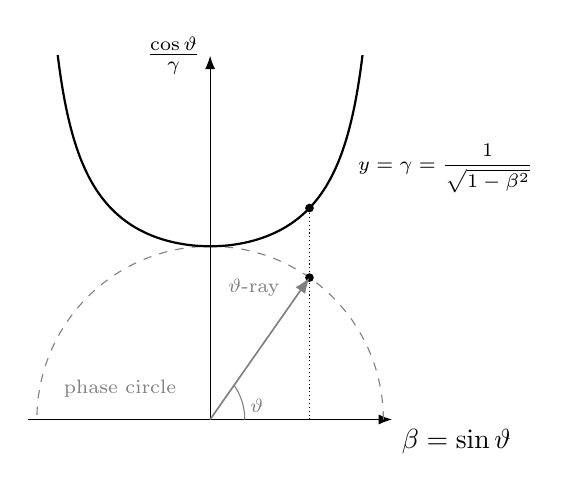
\begin{tikzpicture}[scale=2.2, >=Latex]
  % общие параметры
  \def\ymax{2.1}
  \def\th{35} % пример угла
  \pgfmathsetmacro{\bet}{sin(\th)}   % β = sin θ
  \pgfmathsetmacro{\co}{cos(\th)}    % cos θ
  \pgfmathsetmacro{\ga}{1/\co}       % γ = sec θ

  % оси (вне clip, чтобы надписи не резались)
  \draw[->] (-1.05,0) -- (1.05,0) node[below right] {$\beta=\sin\vartheta$};
  \draw[->] (0,0) -- (0,\ymax) node[left] {$\frac{\cos\vartheta}{ \gamma}$};

  \begin{scope}
    \clip (-1.05,0) rectangle (1.95,\ymax);

    \draw[gray,dashed] (0,0) circle (1);

    \draw[line width=0.8pt] plot[domain=-0.90:0.90, samples=240] (\x, {1/sqrt(1-\x*\x)});

    \draw[densely dotted] (\bet,0) -- (\bet,\ga);
    \fill (\bet,\co) circle (0.025);
    \fill (\bet,\ga) circle (0.025);
  \end{scope}

  \draw[gray,->,line width=0.6pt] (0,0) -- (\bet,\co) node[pos=0.8, above left] {\scriptsize $\vartheta$-ray};
  \draw[gray] (0.20,0) arc[start angle=0, end angle=\th, radius=\th/100];
  \node[gray] at (0.27,0.08) {\scriptsize $\vartheta$};

  \node[gray] at (-0.52,0.18) {\scriptsize phase circle};
  \node at (1.36,1.45) {\scriptsize $y=\gamma=\dfrac{1}{\sqrt{1-\beta^{2}}}$};
\end{tikzpicture}
\caption{Phase circle vs. Lorentz hyperbola at common $\beta=\sin\vartheta$. Vertical mapping at fixed $\beta$ illustrates the Gudermann bridge: $\gamma=\sec\vartheta=\cosh\eta$.}
\label{fig:circle-hyperbola-gd}
\end{figure}
\FloatBarrier

%5 ===================================================================

\section{Time and space as phase derivatives}

Let $\vec{\chi}\in\mathbb{C}$ be a variable whose change generates observable time-space effects. We treat the time and space units as directional derivatives (phase velocities) along the real and imaginary directions of a complex basis $(\hat{h},\mathbf{l})$:
\begin{equation}
\hat{h}\,dx_0=\frac{\partial\vec{\chi}}{\partial\chi_h}\frac{d\chi_h}{d\chi}\,d\chi
=\tilde{H}\,d\chi,\qquad
\mathbf{l}\,dx_l=\frac{\partial\vec{\chi}}{\partial\chi_l}\frac{d\chi_l}{d\chi}\,d\chi
=\tilde{L}\,d\chi,\quad l=1,2,3.
\label{eq:11}
\end{equation}

Introduce the phase speed of the SR interval $ds=\tilde{S}\,d\chi$. The interval conservation takes the form
\begin{equation}
\tilde{S}^2=\frac{ds^2}{d\chi^2}
=\frac{g_{ij}\,dx^i dx^j}{d\chi^2}
=\left( \frac{\mathtt{c} dt}{d\chi} \right)^2 - \left[ \frac{\mathbf{dx}}{d\chi} \right]^2
=\left( \tilde{H} \right)^2 - \left[ \tilde{L} \right]^2,
\label{eq:12}
\end{equation}
equivalently
\begin{equation}
\tilde{H}^2=\tilde{S}^2+\tilde{L}^2.
\label{eq:13}
\end{equation}

Writing 
\begin{equation}
\tilde{S}=\tilde{H}\cos\vartheta,\qquad \tilde{L}=\tilde{H}\sin\vartheta,
\label{eq:14}
\end{equation}
where $\theta$ is the angle of the phase speed relative to the real axis. Algebraically, \eqref{eq:13} is a Euclidean decomposition of a single speed into orthogonal projections; physically, we will see (\ref{subsec:reparam}) that under reparameterization the \emph{projection} $\tilde{S}$, not the Euclidean norm $\tilde{H}$, is the conserved Minkowski quantity.

%6 ===================================================================

\section{Phase space}
Let the flow vector space be $\mathbb{H}$ with orthonormal basis $(\hat{h},\mathbf{l})$. For a flow vector $\boldsymbol{\chi}=R\,e^{\vartheta\mathbf{l}}$ with $\vartheta\in[-\pi,\pi]$,
\begin{equation}
\tilde{H}=R,\qquad \tilde{S}=R\cos\vartheta,\qquad \tilde{L}=R\,\mathbf{l}\sin\vartheta.
\label{eq:21}
\end{equation}

Choosing coordinates where the projectors onto $(\hat{h},\mathbf{l})$ are unit, \eqref{eq:11} simplifies to
\begin{equation}
\hat{h}\,dx_0=\frac{d\chi_h}{d\chi}\,d\chi=\tilde{H}\,d\chi,\qquad
\mathbf{l}\,dx_l=\frac{d\chi_l}{d\chi}\,d\chi=\tilde{L}\,d\chi.
\label{eq:22}
\end{equation}

The map from phase to observables is an integral transform:
\begin{equation}
x^i(\chi)=x^i(\chi_0)+\int_{\chi_0}^{\chi}\tilde{X}^i(u)\,du,\qquad i=0,1,2,3,
\label{eq:23}
\end{equation}
where $\tilde{X}^i$ are projections of $d\boldsymbol{\chi}/d\chi$ onto $(\hat{h},\mathbf{l})$ and $x^i(\chi_0)$ fix initial conditions.

%7 ===================================================================

\section{Objects}
\noindent\textit{Roadmap.} The next formulas fix notation and the geometric carriers we use throughout. In particular, the phase state $(\vartheta,\mathbf u)$ selects a complex slice $\mathbb C_{\mathbf u}\subset\mathbb H$; collinear compositions become ordinary circular sums on this slice, while non-collinear compositions generate a genuine 3D rotation (Wigner–Thomas) via quaternion multiplication. This explains why we keep both $\vartheta$ and $\mathbf u$ as primary objects.

A fundamental particle is an elementary object with nonzero flow $\boldsymbol{\chi}\neq0$. Composite objects are complex flow configurations; to represent them in phase space one may require additional dimensions, except for the photon, whose flow in vacuum is always aligned with the imaginary axis:
\begin{equation}
\mathbf{p}=\frac{d\boldsymbol{\chi}}{d\chi_l}=p\,\mathbf{l}\in\Im.
\label{eq:31}
\end{equation}

Non-photonic phenomena are associated with nonzero real projection and nonzero mass. A complex object can be identified with an event or worldline; the photon corresponds to a null-interval point encoding information about the event.

Any object's phase can be rotated to the \emph{zero} (purely real) direction,
\begin{equation}
\boldsymbol{\chi}_0=R\in\Re.
\label{eq:32}
\end{equation}

An object $A$ moving with speed $\mathbf{v}$ relative to a rest observer has
\begin{equation}
\boldsymbol{\chi}_A=R\,e^{\vartheta_A\mathbf{l}},\qquad
\sin\vartheta_A=\frac{\mathbf{v}}{\mathtt{c}}\equiv\beta.
\label{eq:33}
\end{equation}

\noindent\textit{From unit norm to the interval.}
We will repeatedly use that $cd\tau= c\,dt\,\cos\vartheta$ and $d\mathbf x=c\,dt\,\sin\vartheta\,\mathbf u$.
Thus the identity $\cos^{2}\vartheta+\sin^{2}\vartheta=1$ is exactly the Minkowski metric statement 
$(cd\tau)^{2}=(cdt)^{2}-d\mathbf x^{2}$; from now on, square-root expressions are traded for circular 
trigonometry in $\vartheta$.

%7.1 ===================================================================

\subsection{Space as a symmetric phase pair}
From \eqref{eq:14}, a naive zero-angle limit would remove the imaginary projection, contradicting observability. We enforce a nonvanishing spatial projection by pairing opposite-phase tilts:
\begin{equation}
\boldsymbol{\chi}^{\pm}=R\,e^{\pm\zeta\,\mathbf{l}},\qquad
\boldsymbol{\chi}_l:=\frac{\boldsymbol{\chi}^+-\boldsymbol{\chi}^-}{2}=R\,\mathbf{l}\sin\zeta,
\label{eq:311}
\end{equation}
where $\zeta$ is an internal angle (intrinsic to the object). The local decomposition is
\begin{equation}
\boldsymbol{\chi}_0=\boldsymbol{\chi}_\tau+\boldsymbol{\chi}_l
=R\cos\zeta+R\,\mathbf{l}\sin\zeta,
\label{eq:312}
\end{equation}
with unit components (normalized by $R$): the real component is $\cos\zeta$ and the imaginary component is $\sin\zeta$.

%7.2 ===================================================================

\paragraph{Proper time (geometry).}
Given $(U,\tau,h)$ with $\tau(U)=1$ and $h>0$ on $\ker\tau$, define
\[
g \equiv c^2\,\tau\otimes\tau - h .
\]
The proper time rate for an observer with 4-velocity aligned with $U$ obeys
\[
\frac{d\tau_{\rm proper}}{dt_{\rm lab}} \;=\; \cos\phi \,\cos\vartheta,
\]
where $\cos\vartheta = \gamma^{-1}=\sqrt{1-\beta^2}$ (kinematic) and
$\cos\phi=\sqrt{-g_{00}}$ (gravitational, in a static weak field).


\subsection{Gauge, local, and observed time}
Define \emph{gauge} time $t=t(\tilde{H})$ at the zero phase direction; it is the fastest clock and useful for normalization between different phase speeds. Along the local real direction,
\begin{equation}
dx_0=\frac{d}{d\chi}\Re(\boldsymbol{\chi})\,d\chi
=\frac{\boldsymbol{\chi}^+ + \boldsymbol{\chi}^-}{2}\,d\chi
=\cos\zeta\,d\chi
=:d\tau.
\label{eq:321}
\end{equation}

Here \emph{local} time $d\chi_0:=\cos\zeta\,d\chi$ is the projection of $d\boldsymbol{\chi}$ onto the local real axis; in Sec.~\ref{sec:norm} we calibrate $d\tau=(1/\nu_0)\,d\chi_0$. The \emph{observed} proper time of $A$ relative to the rest observer is
\begin{equation}
\tilde{H}_A=\Re\!\left(\frac{d\boldsymbol{\chi}_A}{d\boldsymbol{\chi}_0}\right)
=\cos\vartheta_A
=\sqrt{1-\sin^2\vartheta_A}
=\sqrt{1-\frac{\mathbf{v}^2}{\mathtt{c}^2}}
=\frac{1}{\gamma}.
\label{eq:322}
\end{equation}



%7.3 ===================================================================

\subsection{Normalization}\label{sec:norm}
\noindent\textit{Calibration.}
We fix the calibration by the observer’s clock and speed budget: $\cos\vartheta \equiv d\tau/dt$ and $\sin\vartheta \equiv \beta$. This choice does not restrict generality: any overall rescaling of the underlying flow is absorbed into the definitions of $t$ and $\mathtt{c}$, leaving all dimensionless observables unchanged.

Let local time be parameterized by flow infinitesimal phase; introduce a reference frequency $\nu_0$ and set
\begin{equation}
d\tau=\frac{1}{\nu_0}\,d\chi_0.
\label{eq:331}
\end{equation}

By the chain rule,
\begin{equation}
dx_0=\tilde{H}\,d\chi
=\frac{dx_0}{d\chi_0}\frac{d\chi_0}{d\tau}\,d\tau
=\tilde{H}\,\dot{\chi}\,d\tau
=: \dot{H}\,d\tau,
\label{eq:332}
\end{equation}
where $\nu:=d\chi/d\tau$, $\dot{\chi}:=\nu/\nu_0$, and $\dot{H}:=\tilde{H}\,\dot{\chi}$. Choosing the calibration $\dot{H}\equiv \mathtt{c}$ gives $dx_0=\mathtt{c}\,d\tau$. Similarly for space,
\begin{equation}
dx_l=\tilde{L}\,d\chi
=\frac{dx_l}{d\chi_0}\frac{d\chi_0}{dl}\,dl
=\tilde{L}\,\chi'\,dl
=:L'\,dl,\qquad \chi':=\frac{d\chi}{dl}.
\label{eq:333}
\end{equation}

From $dx_0=dx_l$ for light one gets
\begin{equation}
\mathtt{c}=\tilde{L}'\,\frac{dl}{d\tau},
\label{eq:334}
\end{equation}
hence with temporal calibration to $\mathtt{c}$ the spatial scale becomes unit: $\tilde{L}'=1$.

%7.4 ===================================================================

\subsection{\texorpdfstring{Light and $\mathtt{c}$ as a calibration constant}{Light and c as a calibration constant}}
From the normalized forms and zero light interval,
\begin{equation}
\frac{\mathtt{c}}{\dot{\chi}}\,d\chi=\frac{1}{\chi'}\,d\chi
\quad\Rightarrow\quad
\mathtt{c}=\frac{\dot{\chi}}{\chi'}=\frac{dl}{d\tau},
\label{eq:341}
\end{equation}
i.e.\ $\mathtt{c}$ is a \emph{calibration constant} tying temporal and spatial measures, independent of local phase variation. Equation \eqref{eq:341} also reads
\begin{equation}
\mathtt{c}=\left(\frac{d\chi}{d\tau}\right)\!\left[\frac{dl}{d\chi}\right]\sim (\nu)\,[\lambda],
\label{eq:343}
\end{equation}
matching frequency and wavelength of a photon, with $\chi$ as its phase. For a lightlike trajectory,
\begin{equation}
ds^2=\mathtt{c}^2\!\left(\frac{d\chi^2}{\dot{\chi}^2}-\frac{d\chi^2}{\dot{\chi}^2}\right)=0.
\label{eq:344}
\end{equation}

At unit frequency, $\tau=\chi$: the photon's ``proper time'' is its phase, and the length of its phase-speed vector equals its wavelength, $\tilde{H}_p=\lambda$. Finally, the kinematic slope in phase coordinates is
\begin{equation}
\frac{dx_l}{dx_0}
=\frac{\tilde{L}\,d\chi}{\tilde{H}\,d\chi}
=\sin\vartheta
=\frac{\mathbf{v}}{\mathtt{c}}
\equiv \beta,
\label{eq:345}
\end{equation}
so $\vartheta=\pi/2$ implies $\mathbf{v}=\mathtt{c}$.

%7.5 ===================================================================

\subsection{Lorentz factor via reparameterization}\label{subsec:reparam}
A change of direction of the flow phase speed transforms
\begin{equation}
\tilde{H}^2=\tilde{S}^2+\tilde{L}^2 \;\longmapsto\;
\dot{H}^2=\dot{S}^2+\dot{L}^2.
\label{eq:351}
\end{equation}
\textbf{Lemma (parameter-change identity).} The transition $\tilde{H}\to\dot{S}$ is the manifestation of evolving flow phase speed under the parameter change $\chi\mapsto \tau(\chi)$, with local Jacobian
\begin{equation}
\frac{d\tau}{d\chi}=\cos\zeta(\chi)\cos\vartheta(\chi)
\quad\Rightarrow\quad
\mathcal{J}(\zeta,\vartheta):=\frac{d\chi}{d\tau}=\frac{1}{\cos\zeta\,\cos\vartheta}.
\label{eq:353}
\end{equation}

Then
\begin{equation}
\dot{H}=\tilde{H}\,\mathcal{J},\qquad \dot{L}=\tilde{L}\,\mathcal{J}.
\label{eq:354}
\end{equation}

In differential form,
\begin{equation}
d\ln\dot{H}=d\ln\mathcal{J}=\tan\zeta\,d\zeta+\tan\vartheta\,d\vartheta.
\label{eq:355}
\end{equation}

For a pure boost ($d\zeta=0$) one has $d\dot{H}=\dot{H}\tan\vartheta\,d\vartheta$. Absorbing a constant $\cos\zeta$ into the calibration (set $\zeta=0$ henceforth), we obtain
\begin{equation}
\tilde{H}^2=\dot{H}^2-\dot{L}^2=\sec^2\vartheta\,(\tilde{H}^2-\tilde{L}^2)=\gamma^2(\tilde{H}^2-\tilde{L}^2).
\label{eq:356}
\end{equation}
\textbf{Corollary.} In phase space the Euclidean norm $\tilde{H}$ is conserved; in observed time the Minkowski norm $\dot{S}$ is conserved; they are identical as quantities:
\begin{equation}
\boxed{\ \tilde{H}=\dot{S}\ }.
\label{eq:357}
\end{equation}

%7.6 ===================================================================

\subsection{Rapidity and the phase angle}
By definition,
\begin{equation}
\beta=\frac{\mathbf v}{\mathtt{c}}=\sin\vartheta,\qquad \tanh\eta=\beta,\qquad
d\eta=\frac{d\beta}{1-\beta^2}.
\label{eq:361}
\end{equation}

With $d\beta=\cos\vartheta\,d\vartheta$ and $1-\beta^2=\cos^2\vartheta$,
\begin{equation}
d\eta=\sec\vartheta\,d\vartheta,\qquad
\eta(\vartheta)=\int\sec\vartheta\,d\vartheta
=\ln|\sec\vartheta+\tan\vartheta|
=\tfrac12\ln\frac{|1+\sin\vartheta|}{|1-\sin\vartheta|}.
\label{eq:364}
\end{equation}

Fixing $\eta(0)=0$,
\begin{equation}
e^{\eta(\vartheta)}=\sqrt{\frac{1+\sin\vartheta}{1-\sin\vartheta}},\qquad
\gamma=\frac{1}{\sqrt{1-\beta^2}}=\sec\vartheta=\cosh\eta.
\label{eq:365}
\end{equation}

\paragraph{Remark (groups).} Observables satisfy $\beta=\sin\vartheta=\tanh\eta$ and $\gamma=\sec\vartheta=\cosh\eta$. Thus Euclidean rotations in the phase circle (\,$U(1)$ with angle $\vartheta$\,) reproduce the numerical factors of hyperbolic boosts in $SO^+(1,1)$ (rapidity $\eta$) after reparameterizing time. We do not claim an isomorphism $U(1)\cong SO(1,1)$; only the equality of observable combinations under the change of parameter.

%7.7 ===================================================================

\subsection{Velocity addition}
\label{sec:vel-addition}

\paragraph{Notation.}
In unimetry, an inertial boost is a \emph{D-rotation}
\begin{equation}
\label{eq:auto:32}
\mathcal{B}(\uhat,\psi):\quad \mathbf q \mapsto d\,\mathbf q\,d,
\qquad
d=\cos\frac{\psi}{2}+\uhat\,\sin\frac{\psi}{2},
\end{equation}
and a spatial rotation is an \emph{R-rotation}
\begin{equation}
\label{eq:auto:33}
\mathcal{R}(\hat{\mathbf n},\varphi):\quad \mathbf q \mapsto r\,\mathbf q\,r^{-1},
\qquad
r=\cos\frac{\varphi}{2}+\hat{\mathbf n}\,\sin\frac{\varphi}{2}.
\end{equation}

Kinematic mapping: $\beta\equiv \mathbf v/ \mathtt c=\sin\psi$, $\gamma=1/\cos\psi$,
$\displaystyle \tan\frac{\psi}{2}=\frac{\gamma\beta}{\gamma+1}$.
For quaternionic/GA accounts of rotors and Lorentz boosts see \cite{Hamilton1844,HestenesSobczyk1984,DoranLasenby2003}.

\subsubsection{Wigner rotation}
\label{subsec:wigner}

Let $d_1,d_2$ be D-rotors of two successive boosts. The raw action on any unimetry 4-object is
\begin{equation}
\label{eq:auto:34}
\mathbf q' = d_2 d_1\, \mathbf q\, d_1 d_2 \equiv L_{12}\,\mathbf q\,L_{21},\qquad
L_{12}=d_2 d_1,\ \ L_{21}=d_1 d_2.
\end{equation}

Define $d_{12}$ to be the unique D-rotor reproducing the combined spatio--temporal tilt of $L_{12}$:
\begin{equation}
\boxed{\, d_{12}\,\mathbf e_t\, d_{12} \;=\; L_{12}\,\mathbf e_t\, L_{21},\qquad \Re(d_{12})\ge0 \,}
\label{eq:d12-uniqueness}
\end{equation}
(the sign choice removes the trivial two-fold ambiguity). Then the Wigner rotor is the residual
R-rotation in the symmetric D--R factorization:
\begin{equation}
\boxed{\, L_{12}=d_{12}\,r_W,\qquad L_{21}=r_W^{-1}\,d_{12} \,}
\label{eq:DR-polar}
\end{equation}
equivalently,
\begin{equation}
\boxed{\, r_W=\bar d_{12}\,L_{12}=L_{21}\,\bar d_{12} \,}.
\label{eq:wigner-rotor-def}
\end{equation}

Hence the observed map after compensating the tilt is $\,\bar d_{12}\,\mathbf q'\,\bar d_{12}=r_W\,\mathbf q\,r_W^{-1}$.

\begin{figure}[!ht]
\centering
\begin{tikzpicture}[>=Latex, node distance=32mm]
  \node (q) {$\mathbf q$};
  \node (d1) [right=of q] {$d_1\,\mathbf q\,d_1$};
  \node (d2) [right=of d1] {$d_2 d_1\,\mathbf q\,d_1 d_2$};
  \node (rw) [below=20mm of d2] {$r_W\,\mathbf q\,r_W^{-1}$};
  \draw[->] (q) -- node[above] {$d_1$} (d1);
  \draw[->] (d1) -- node[above] {$d_2$} (d2);
  \draw[->] (d2) -- node[right] {$\bar d_{12}$ on both sides} (rw);
  \draw[->, dashed, bend left=12] (q) to node[above] {$d_{12}$} (d2);
\end{tikzpicture}
\caption{Two successive D-rotations (boosts) and compensation of the net spatio--temporal angle by the conjugate of $d_{12}$, leaving a pure R-rotation $r_W$.}
\label{fig:tikz-wigner-pullback}
\end{figure}

\subsubsection{Thomas precession}
\label{subsec:thomas}
The continuous limit of Wigner rotation for a time-dependent velocity direction $\uhat(t)$ yields
\begin{equation}
\label{eq:auto:38}
\boldsymbol{\omega}_T=(\gamma-1)\,\bigl(\uhat\times \dot{\uhat}\bigr)
=\frac{\gamma^2}{\gamma+1}\,\frac{\mathbf a\times \mathbf v}{c^2},\qquad
\gamma=\frac{1}{\cos\psi}.
\end{equation}

For uniform circular motion ($|\mathbf v|=\mathrm{const}$) with $\dot{\uhat}=\boldsymbol{\Omega}\times\uhat$ one has
$\lvert\boldsymbol{\omega}_T\rvert=(\gamma-1)\,\Omega$.

%7.8 ===================================================================

\subsection{Doppler shift}
Define the observed frequency as the phase growth rate in the observer's proper time:
\begin{equation}
\nu:=\frac{d\chi}{d\tau}.
\label{eq:381}
\end{equation}

For two successive wavefronts the phase increment is identical, hence
\begin{equation}
\frac{\nu_{\mathrm{obs}}}{\nu_{\mathrm{src}}}
=\frac{d\chi/d\tau_{\mathrm{obs}}}{d\chi/d\tau_{\mathrm{src}}}
=\frac{d\tau_{\mathrm{src}}}{d\tau_{\mathrm{obs}}}.
\label{eq:382}
\end{equation}

Longitudinal case: during $\gamma\,d\tau_{\mathrm{src}}$ in the observer frame the source displaces by $\pm \mathbf v\,\gamma\,d\tau_{\mathrm{src}}$ (``$+$'' receding, ``$-$'' approaching). Then
\begin{equation}
d\tau_{\mathrm{obs}}=\gamma\,d\tau_{\mathrm{src}}(1\pm\beta),\qquad
\Rightarrow\quad
\boxed{\ \frac{\nu_{\mathrm{obs}}}{\nu_{\mathrm{src}}}=\frac{1}{\gamma(1\pm\beta)}\ }.
\label{eq:384}
\end{equation}

Equivalent forms (with $\beta=\sin\vartheta$, $\gamma=\sec\vartheta$ and rapidity $\eta$):
\begin{equation}
\frac{\nu_{\mathrm{obs}}}{\nu_{\mathrm{src}}}
=\sqrt{\frac{1\mp\beta}{1\pm\beta}}
=\sec\vartheta\,(1\mp\sin\vartheta)
=e^{\mp\eta}.
\label{eq:385}
\end{equation}

Transverse Doppler ($\varphi=90^\circ$ in the observer's frame):
\begin{equation}
\frac{\nu_{\mathrm{obs}}}{\nu_{\mathrm{src}}}=\frac{1}{\gamma}=\cos\vartheta.
\label{eq:389}
\end{equation}

General line-of-sight (LOS) angle $\varphi$ in the observer's frame:
\begin{equation}
\boxed{\ \frac{\nu_{\mathrm{obs}}}{\nu_{\mathrm{src}}}=\gamma\,(1-\beta\cos\varphi)\ }.
\label{eq:3810}
\end{equation}

Wavelength ratios are inverse to frequency ratios.

%8 ===================================================================

\section{Unified temporal effects in phase space}
\label{ch:optics}

We factor all time-related effects through a single phase tilt structure.
Let the intrinsic (\(\zeta\)), gravitational (\(\phi\)), and kinematic (\(\vartheta\)) angles be independent contributors to the phase tilt at a point.
Define the local \emph{time-rate factor}
\begin{equation}
\label{eq:time-rate-factor}
\frac{d\tau}{dt}
\;=\;
\cos\zeta\;\cos\phi\;\cos\vartheta,
\qquad
n_{\rm tot}\;:=\;\sec\zeta\;\sec\phi\;\sec\vartheta,
\end{equation}
where \(n_{\rm tot}\) plays the role of an effective (phase) refractive index for light propagation.
Accordingly, the coordinate light-travel time along a spatial curve \(\Gamma\) is
\begin{equation}
\label{eq:optical-length}
t_\Gamma \;=\; \frac{1}{\mathtt c}\int_\Gamma n_{\rm tot}\,ds.
\end{equation}

\paragraph{Lemma (Unified time-rate).}
In the unimetry phase representation, the proper-to-lab time rate and the optical length factorize as in \eqref{eq:time-rate-factor}–\eqref{eq:optical-length}.
Setting any subset of angles to zero recovers the corresponding standard effects:
\begin{itemize}\itemsep4pt
  \item \textbf{Special relativity (vacuum SR):} \(\zeta=0,\ \phi=0\Rightarrow d\tau/dt=\cos\vartheta=1/\gamma\) (kinematic time dilation).
  \item \textbf{Gravitational clocks (static weak field):} \(\zeta=0,\ \vartheta=0\Rightarrow d\tau/dt=\cos\phi\) (gravitational redshift/clock rate); calibration of \(\phi\) reproduces the usual \(\sqrt{g_{00}}\).
  \item \textbf{Shapiro delay (gravitational contribution to TOF):} with \(\zeta=0,\ \vartheta=0\), \eqref{eq:optical-length} yields \(t_\Gamma=(1/\mathtt c)\int \sec\phi\,ds\); the excess over \(\int ds/\mathtt c\) is the Shapiro time delay.
  \item \textbf{Intrinsic/evolutionary tilt:} \(\phi=0,\ \vartheta=0\Rightarrow d\tau/dt=\cos\zeta,\ n_{\rm tot}=\sec\zeta\) (useful as a time gauge in cosmological/effective-medium contexts).
\end{itemize}

\paragraph{Remarks.}
(i) The factorization in \eqref{eq:time-rate-factor} is the phase-space counterpart of composing independent tilts; it preserves the conserved Minkowski norm once time is reparameterized by \(\tau\).
(ii) For vacuum SR we simply set \(\zeta=0\) and work with \(\vartheta\); for pure gravitational timing we set \(\vartheta=0\) and use \(\phi\).
(iii) Non-collinear boost composition acts on \(\vartheta\) via quaternionic rotors and induces a Wigner/Thomas residual \emph{spatial} rotation without altering \eqref{eq:time-rate-factor}.

\section{\texorpdfstring{Gravity as a phase rotation: local tetrads and clock angle}{Gravity as a phase rotation}}

On a curved background $(\mathcal M,g)$ we work with orthonormal tetrads $e_a{}^\mu$ such that $g_{\mu\nu}e_a{}^\mu e_b{}^\nu=\eta_{ab}$ and take the observer's time leg to be $e_0{}^\mu$. 
We introduce the \emph{gravitational (clock) angle} $\varphi$ by
\begin{equation}
\cos\varphi\ :=\ e^0{}_\mu\,u^\mu\ =\ \frac{d\tau_{\rm stat}}{dt}\ =\ \sqrt{-g_{00}}\qquad\text{(stationary case)}.
\label{eq:clock-angle}
\end{equation}

Kinematics remains encoded by the phase angle $\vartheta$ in the slice $\mathbb C_{\mathbf u}$, with
$\cos\vartheta=d\tau/d\tau_{\rm stat}$. 
Therefore the proper time factorizes as
\begin{equation}
d\tau\ =\ dt\,\cos\varphi\,\cos\vartheta,\qquad 
d\mathbf x\ =\ c\,dt\,\sin\vartheta\,\mathbf u,
\label{eq:tau-factorization}
\end{equation}
and the total redshift factorizes into kinematic and gravitational parts:
\begin{equation}
1+z_{\rm tot}\ =\ \frac{\cos\vartheta_{\rm em}}{\cos\vartheta_{\rm obs}}\ \times\ 
\frac{\cos\varphi(x_{\rm em})}{\cos\varphi(x_{\rm obs})}.
\label{eq:z-factorization}
\end{equation}

For static emitter/observer ($\vartheta_{\rm em}=\vartheta_{\rm obs}=0$) one recovers the standard gravitational redshift 
$1+z_g=\sqrt{\frac{-g_{00}(x_{\rm obs})}{-g_{00}(x_{\rm em})}}$.
In the weak-field limit $g_{00}\simeq-(1+2\Phi/c^2)$ this gives $z_g\simeq(\Phi_{\rm obs}-\Phi_{\rm em})/c^2$.

\paragraph{Beyond static fields.}
In a $3\!+\!1$ split $ds^2=-N^2 c^2 dt^2 + h_{ij}(dx^i+N^i dt)(dx^j+N^j dt)$ one may identify $\cos\varphi:=N$ in the observer's tetrad, which keeps \eqref{eq:tau-factorization}–\eqref{eq:z-factorization} coordinate-agnostic.
Uniform acceleration (Rindler) accumulates phase according to $d\vartheta=\kappa\,dt$ inside the local slice, consistently reproducing accelerated-frame kinematics when combined with the clock angle $\varphi$.

%9 ===================================================================

\section{Discussion: links to known structures}

\paragraph{Gauge phases.} A global shift $\chi\mapsto\chi+\chi_0$ is unobservable. Allowing local reparameterizations $\chi\mapsto\chi+\alpha(x)$ induces a connection when comparing phases at different points. On wavefunctions $\psi\sim e^{i\chi}$ this is the familiar $U(1)$ gauge freedom $\psi\to e^{i\alpha(x)}\psi$ with $D_\mu=\partial_\mu-iA_\mu$ as the \emph{phase-transport connection}.

\paragraph{Mass and the internal angle.} With the decomposition by $\zeta$, mass heuristically correlates with an irreducible real projection: massless objects have $\zeta=\pm\pi/2$ (no proper time; photon subspace), while massive objects have $|\zeta|<\pi/2$ (proper time exists). A detailed mass-generation mechanism is left for future work.

\paragraph{Cosmological gauge.} A natural global calibration of ``absolute'' time is the comoving frame with vanishing CMB dipole. This fixes a cosmological time $t$ (FLRW) as a gauge, without affecting local Lorentz invariance; Doppler factors are then operationally referenced to that frame.

\section{Conclusion}
In unimetry, time and space are integrals of phase velocities; the Minkowski interval appears as a conserved quantity under parameter change. The core relations of SR---$\gamma$, rapidity, velocity addition, and Doppler factors---follow from elementary phase-plane geometry with a single rotation angle $\theta$, while hyperbolic structure re-emerges upon reparameterizing time. The formalism is empirically equivalent to standard SR but can clarify causality and composition by treating all effects as projections of a single flow.

\paragraph{Outlook.} Future directions include (i) a more explicit group-theoretic embedding, (ii) a rigorous treatment of the internal angle $\zeta$ and its relation to mass, and (iii) exploration of curved metrics as spatially varying Jacobians $\mathcal{J}(x)$ in the phase-to-observable map.

\bibliographystyle{plain}
\begin{thebibliography}{9}
\bibitem{Gudermann1830}  NIST Digital Library of Mathematical Functions, §4.23 ``Gudermannian Function'', \url{https://dlmf.nist.gov/4.23}.

\bibitem{Hopf1931}
H.~Hopf, ``Über die Abbildungen der dreidimensionalen Sphäre auf die Kugelfläche,'' \emph{Mathematische Annalen} \textbf{104} (1931) 637--665. \href{https://doi.org/10.1007/BF01457962}{doi:10.1007/BF01457962}.

\bibitem{Thomas1926}
L.~H.~Thomas, ``The Motion of the Spinning Electron,'' \emph{Nature} \textbf{117} (1926) 514. \href{https://doi.org/10.1038/117514a0}{doi:10.1038/117514a0}.

\bibitem{Wigner1939}
E.~P.~Wigner, ``On Unitary Representations of the Inhomogeneous Lorentz Group,'' \emph{Annals of Mathematics} \textbf{40} (1939) 149--204. \href{https://doi.org/10.2307/1968551}{doi:10.2307/1968551}.
\bibitem{Berry1984}
M.~V.~Berry, ``Quantal phase factors accompanying adiabatic changes,'' \emph{Proceedings of the Royal Society A} \textbf{392} (1984) 45--57. \href{https://doi.org/10.1098/rspa.1984.0023}{doi:10.1098/rspa.1984.0023}.

\bibitem{Shapiro1964}
I.~I.~Shapiro, ``Fourth Test of General Relativity,'' \emph{Phys. Rev. Lett.} \textbf{13} (1964) 789--791. \href{https://doi.org/10.1103/PhysRevLett.13.789}{doi:10.1103/PhysRevLett.13.789}.

\bibitem{RindlerBook}
W.~Rindler, \emph{Relativity: Special, General, and Cosmological}, 2nd ed., Oxford University Press, 2006.

\bibitem{MTW}
C.~W.~Misner, K.~S.~Thorne, J.~A.~Wheeler, \emph{Gravitation}, W.~H.~Freeman, 1973.

\bibitem{Jackson}
J.~D.~Jackson, \emph{Classical Electrodynamics}, 3rd ed., Wiley, 1999.

\bibitem{Einstein1905}
A.~Einstein.
\newblock Zur Elektrodynamik bewegter K\"{o}rper.
\newblock {\em Annalen der Physik}, 17:891--921, 1905.
(English translation: On the electrodynamics of moving bodies.)

\bibitem{Rindler}
W.~Rindler.
\newblock {\em Relativity: Special, General, and Cosmological}.
\newblock Oxford University Press, 2nd ed., 2006.

\bibitem{TaylorWheeler}
E.~F. Taylor and J.~A. Wheeler.
\newblock {\em Spacetime Physics}.
\newblock W. H. Freeman, 2nd ed., 1992.

\bibitem{Hamilton1844}
W.~R.~Hamilton,
\newblock \emph{On quaternions; or on a new system of imaginaries in algebra}, Philosophical Magazine \textbf{25}, 10--13 (1844).

\bibitem{HestenesSobczyk1984}
D.~Hestenes and G.~Sobczyk,
\newblock \emph{Clifford Algebra to Geometric Calculus}, Reidel, 1984.

\bibitem{DoranLasenby2003}
C.~Doran and A.~Lasenby,
\newblock \emph{Geometric Algebra for Physicists}, Cambridge University Press, 2003.

\end{thebibliography}




\appendix
\section{Equivalence to the classical Wigner rotation}
\label{app:1}

We sketch an intrinsic quaternionic proof that the unimetry expression for the Wigner rotation
coincides with the standard special-relativistic formula.

\paragraph{Step 1: product of two D-rotors.}
For $d_i=\cos\frac{\psi_i}{2}+\uhat_i\sin\frac{\psi_i}{2}$,
\begin{equation}
\label{eq:auto:45}
d_2 d_1
=(c_2c_1-s_2s_1\cos\theta)
+\Big(c_2s_1\uhat_1+s_2c_1\uhat_2+s_2s_1\,\uhat_2\times\uhat_1\Big),
\end{equation}
with $c_i=\cos(\psi_i/2)$, $s_i=\sin(\psi_i/2)$ and $\cos\theta=\uhat_2\!\cdot\!\uhat_1$.

\paragraph{Step 2: symmetric D--R factorization.}
Define $d_{12}$ by $d_{12}\,\mathbf e_t\, d_{12}=L_{12}\,\mathbf e_t\, L_{21}$ and set
$r_W=\bar d_{12}\,L_{12}=L_{21}\,\bar d_{12}$. Then $r_W$ fixes $\mathbf e_t$ and is a pure spatial
rotor, so $r_W=\cos\frac{\phi}{2}+\hat{\mathbf n}\sin\frac{\phi}{2}$ with
$\hat{\mathbf n}\parallel \uhat_2\times\uhat_1$. Matching scalar and bivector parts gives
\begin{equation}
\tan\frac{\phi}{2}=
\frac{s_1 s_2\,\sin\theta}{\,c_1 c_2+s_1 s_2\,\cos\theta\,}.
\label{eq:uni-phi}
\end{equation}

\paragraph{Step 3: map to rapidities.}
With the substitutions $\sin(\psi/2)\mapsto\sinh(\eta/2)$, $\cos(\psi/2)\mapsto\cosh(\eta/2)$,
$\tan(\psi/2)\mapsto\tanh(\eta/2)$ (where $\tanh\eta=\beta$, $\cosh\eta=\gamma$), \eqref{eq:uni-phi}
becomes the textbook Wigner angle:
\begin{equation}
\label{eq:auto:47}
\tan\frac{\phi}{2}
=\frac{\sinh\frac{\eta_1}{2}\,\sinh\frac{\eta_2}{2}\,\sin\theta}
{\cosh\frac{\eta_1}{2}\,\cosh\frac{\eta_2}{2}+\sinh\frac{\eta_1}{2}\,\sinh\frac{\eta_2}{2}\,\cos\theta},
\end{equation}
with axis along $\uhat_2\times\uhat_1$. This circular--hyperbolic correspondence is classical; cf.\ Gudermann~\cite{Gudermann1830}.

\section{A worked example — Wigner angle in hyperbolic vs phase parametrizations with a stability note}\label{app:wigner}
\label{app:2}

\paragraph{Closed-form formulae.}
Let $\boldsymbol\beta_i$ ($i=1,2$) be two non-collinear boost velocities with magnitudes $\beta_i=\|\boldsymbol\beta_i\|<1$ and let $\chi$ be the angle between their \emph{directions}.
The Thomas–Wigner rotation $R_W$ generated by the composition of boosts has axis
$\hat{\mathbf n}\parallel \hat{\boldsymbol\beta}_2\times \hat{\boldsymbol\beta}_1$
and angle $\psi_W$ given by either of the following equivalent half–angle forms:
\begin{align}
\tan\frac{\psi_W}{2}
&=\frac{\sin\chi\;\tanh\!\frac{\eta_1}{2}\;\tanh\!\frac{\eta_2}{2}}
       {1+\cos\chi\;\tanh\!\frac{\eta_1}{2}\;\tanh\!\frac{\eta_2}{2}} ,
\qquad \beta_i=\tanh\eta_i ,
\label{eq:wigner-hyp}\\[4pt]
\tan\frac{\psi_W}{2}
&=\frac{\sin\chi\;\tan\!\frac{\vartheta_1}{2}\;\tan\!\frac{\vartheta_2}{2}}
       {1+\cos\chi\;\tan\!\frac{\vartheta_1}{2}\;\tan\!\frac{\vartheta_2}{2}} ,
\qquad \beta_i=\sin\vartheta_i .
\label{eq:wigner-phase}
\end{align}
Numerically stable and parametrization–agnostic is the identity
\begin{equation}
\tanh\!\frac{\eta_i}{2}=\tan\!\frac{\vartheta_i}{2}
=\frac{\gamma_i\beta_i}{1+\gamma_i}
=\frac{\beta_i}{\,1+\sqrt{1-\beta_i^2}\,}
=:t_i ,
\qquad \gamma_i=(1-\beta_i^2)^{-1/2}.
\label{eq:half-angle-t}
\end{equation}
With $t_i$ from \eqref{eq:half-angle-t}, both \eqref{eq:wigner-hyp}–\eqref{eq:wigner-phase} reduce to
\begin{equation}
\psi_W
=2\,\operatorname{atan2}\!\Big(\sin\chi\,t_1t_2,\;1+\cos\chi\,t_1t_2\Big),
\label{eq:wigner-atan2}
\end{equation}
which avoids overflow/underflow and ensures the correct quadrant.

\paragraph{Example A (orthogonal boosts, moderate $\gamma$).}
Take $\boldsymbol\beta_1=(0.8,0,0)$ and $\boldsymbol\beta_2=(0,0.6,0)$, so $\chi=\pi/2$.
From \eqref{eq:half-angle-t} one finds $t_1=\tfrac{1}{2}$ and $t_2=\tfrac{1}{3}$ exactly,
hence $\tan(\psi_W/2)=t_1t_2=\tfrac{1}{6}$ and
\[
\boxed{\;\psi_W
=2\arctan\!\frac{1}{6}
=0.3302973548292537~\text{rad}
=18.924644416051237^\circ\;}
\]
Both parametrizations \eqref{eq:wigner-hyp} and \eqref{eq:wigner-phase} coincide to machine precision.
A direct $4{\times}4$ Lorentz–matrix composition followed by polar decomposition of the spatial block
recovers $\psi_W=0.3302973548292533$ rad (agreement to $<5{\times}10^{-16}$ rad).

\paragraph{Example B (ultra–relativistic, small inter–direction angle).}
Let $\boldsymbol\beta_1=(0.999999,0,0)$ and
$\boldsymbol\beta_2=0.9999(\cos 1^\circ,\sin 1^\circ,0)$ so that $\chi=1^\circ$.
Then \eqref{eq:half-angle-t} gives $t_1=0.9985867853779378$, $t_2=0.9859568136154433$ and
\[
\boxed{\;\psi_W
=2\,\operatorname{atan2}\!\big( \sin1^\circ\;t_1t_2,\;1+\cos1^\circ\;t_1t_2\big)
=0.0173175319077011~\text{rad}
=0.9922214898944112^\circ\;}
\]
The same value is obtained from either \eqref{eq:wigner-hyp} or \eqref{eq:wigner-phase}.
A double–precision Lorentz–matrix calculation with orthonormalization of the spatial block yields
$\psi_W=0.0173175044768120$ rad (agreement to $\sim 3{\times}10^{-8}$ rad; the residual is purely numerical).

\paragraph{Stability and accumulated error (practical note).}
\begin{itemize}
\item \textbf{Half–angle is key.} Computing via \eqref{eq:half-angle-t} and \eqref{eq:wigner-atan2} is markedly more stable than
naively evaluating $\eta_i=\operatorname{artanh}\beta_i$ followed by $\sinh(\eta_i/2),\cosh(\eta_i/2)$,
especially for $\gamma\gtrsim 10^2$ or tiny $\chi$ where subtractive cancellation appears in the denominator of \eqref{eq:wigner-hyp}.
\item \textbf{Single vs double precision.}
For Example~A, all routes (phase/hyperbolic/matrix) agree within $\sim 10^{-7}$ rad even in single precision.
For Example~B, the analytic half–angle formula \eqref{eq:wigner-atan2} remains well-behaved in single precision
($\psi_W=0.01731725$ rad; deviation $\sim 3{\times}10^{-7}$ rad),
while a direct $4{\times}4$ matrix composition in single precision becomes ill–conditioned (eigen–based orthonormalization fails to converge), a manifestation of catastrophic rounding at $\gamma\sim 10^3$.
\item \textbf{Error accumulation under repetitions.}
If the same pair of boosts is applied repeatedly, the rotation axis $\hat{\mathbf n}$ is fixed and the angle adds linearly mod $2\pi$.
In finite precision, composing dense Lorentz matrices $N$ times amplifies roundoff roughly linearly in $N$,
whereas evaluating \eqref{eq:wigner-atan2} per step and accumulating the angle avoids the growth of matrix–multiplication conditioning.
\end{itemize}

\paragraph{Recommendation (for reproducible numerics).}
Use \eqref{eq:half-angle-t} to form $t_i$ directly from $\beta_i$, then evaluate \eqref{eq:wigner-atan2} with \texttt{atan2}.
When a matrix route is unavoidable, extract the spatial rotation by removing the net boost and projecting the $3{\times}3$ block to $\mathrm{SO}(3)$ via a polar decomposition before reading off $\psi_W$.


\end{document}
